\subsection{Гидрологический цикл. Конденсация и туманы. Облака.}
\textit{Конденсация} –- процесс перехода воды из газообразного состояния в жидкое при понижении температуры до точки росы\footnote{Точка росы -- температура, при которой водяной пар становится насыщенным.}.

\textit{Гидрологический цикл} (круговорот воды в природе) можно описать следующим образом: вода, находящаяся в жидком состоянии, испаряется, поднимается в атмосферу, где конденсируется, образуя облака или туманы, а в дальнейшем снова возвращается на землю уже в жидком состоянии в виде дождя или росы, либо через промежуточные твёрдые состояния – снег, иней, град.

\textit{Облака} –- взвешенные в атмосфере продукты конденсации водяного пара.
Облака образуются при адиабатическом охлаждении воздуха.

Виды облаков по высоте (см. рис. \ref{fig:clouds}):
\begin{enumerate}
\item Облака верхнего яруса (> 6 км).
\item Облака среднего яруса (2--6 км).
\item Облака нижнего яруса (< 2 км).
\end{enumerate}

\begin{figure}[!ht]
\centering
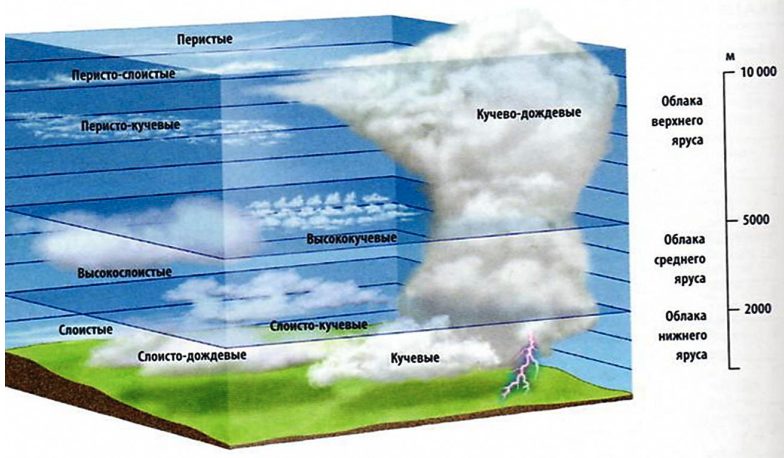
\includegraphics[width=0.5\textwidth]{images/clouds.png}
\caption{Виды облаков.}\label{fig:clouds}
\end{figure}

Виды облаков по происхождению:
\begin{enumerate}
\item Фронтальные облака. Образуются при подъёме тёплого воздуха по холодному.
\item Орографические облака. Образуются при обтекании воздуха возвышенностей рельефа.
\end{enumerate}

\textit{Туман} -- взвешенные продукты конденсации водяного пара непосредственно над поверхностью Земли.
Физически механизм образования туманов (так же, как и облаков) под влиянием горизонтального перемешивания можно представить в следующем виде.
Если смешиваются два объёма воздуха с различной температурой, то температура тёплого воздуха понижается. Избыток водяного пара (сверх насыщения) в тёплом воздухе при этом конденсируется.
Затем капли воды распространяются на весь объём.
Так как в холодном воздухе температура при этом повышается, то в нём возникает недостаток насыщения: часть капель, поэтому испаряется, а оставшаяся масса капель образует туман.
